\section{Main Results}
\label{sec:results}

\subsection{Overall Effectiveness (RQ1)}
Table~\ref{tab:overall} reports end-to-end performance on the core multi-hop
QA workloads (HotpotQA, 2WikiMultiHopQA, MuSiQue) under the matched-budget
protocol of Section~\ref{sec:experiments}. Across all three datasets the
requirement-aware optimizer (\code{slotrag-g7-chain}) matches or beats the
frozen static baseline on exact-match: HotpotQA $37.5\%\to43.8\%$
($\Delta{=}{+}6.3$pt), 2Wiki $52.9\%\to58.8\%$ ($\Delta{=}{+}5.9$pt), and
MuSiQue $36.4\%\to45.5\%$ ($\Delta{=}{+}9.1$pt), with a pooled
$+7.3$pt on 55 matched questions. These gains are uniformly positive but
\emph{not} statistically supported: the McNemar exact test on discordant pairs
finds at most three chain-favoring flips (HotpotQA $2{:}1$, 2Wiki $3{:}2$,
MuSiQue $3{:}1$), all with $p\geq 0.625$, and the pooled EM bootstrap interval
$[-5.5,+20.0]$pt includes zero. We therefore do \emph{not} claim an EM win on
any dataset; the honest statement is a consistent, directionally positive but
statistically inconclusive EM difference on the model this paper uses
(qwen3.8-27b). Figure~\ref{fig:overall-em} visualizes the per-dataset EM
comparison.

The chain arm's second effect is cost. Realized retrieval calls drop on every
dataset---HotpotQA $-0.19$, 2Wiki $-0.24$, MuSiQue $-0.09$ calls/question,
pooled $-0.16$---but none of these reductions is significant at the
single-test or Holm-adjusted level ($p_{\text{boot}}\in[0.119,0.376]$;
$p_{\text{Holm}}$ up to $0.581$). Under the current (cheap, 1--2 call)
operating point, the chain's savings are small in absolute terms and are
swamped by per-question variance, so we report them as a uniform but
\emph{not statistically supported} cost reduction. The savings concentrate
where the chain law leaves allocation freedom---the $\ge 3$-slot subdomain
(pooled $-1.09$ calls/question, bootstrap $p=0.036$, CI $[-2.18,+0.09]$), at
pooled EM difference exactly zero. The $1$--$2$-slot chains that dominate most QA
splits are close to their chain-law budget floor, so the optimizer has little to
save there; the per-question differences on those chains are small and not
uniform in direction.

Taken together, the honest boundary is: on the full matched sample the chain
arm delivers directionally positive but statistically inconclusive EM gains
and a uniform but not significant cost reduction; on the $\ge 3$-slot
subdomain---where the optimizer has genuine degrees of freedom---the cost
saving is larger and the EM difference is exactly zero. This is a weaker but
more honest claim than the earlier model's ``cost-only'' finding: with the
model switch the cost advantage shrank below significance while EM differences
turned positive.

\begin{table}[t]
\centering
\caption{End-to-end matched-budget evaluation across three multi-hop QA
datasets (development/validation split, seed $2027$). Retrieval budget $=8$;
method: chain-rule importance ($\tau = 2d - 1$); plan: frozen across arms.
$\Delta$ is chain $-$ static. Compiled slot counts (from stored plans): HotpotQA
1-slot $=13$, 2-slot $=2$, $\ge 3$-slot $=5$; 2Wiki
1-slot $=9$, 2-slot $=4$, $\ge 3$-slot $=7$; MuSiQue 1-slot $=13$,
2-slot $=3$, $\ge 3$-slot $=7$ (plus one 0-slot plan). Hop label $\ne$ compiled slot count.}
\label{tab:overall}
\small
\begin{tabular}{lrcccccc}
\toprule
dataset & \#q & EM$_{\text{static}}$ & EM$_{\text{chain}}$ & $\Delta$EM & $\Delta$calls & $p_{\text{boot}}$ & $p_{\text{Holm}}$ \\
\midrule
HotpotQA  & 16 & 37.5\% & 43.8\% & $+6.3$ & $-0.19$ & 0.119 & 0.357 \\
2Wiki     & 17 & 52.9\% & 58.8\% & $+5.9$ & $-0.24$ & 0.290 & 0.581 \\
MuSiQue   & 22 & 36.4\% & 45.5\% & $+9.1$ & $-0.09$ & 0.376 & 0.376 \\
\midrule
\textsc{All}    & 55 & 41.8\% & 49.1\% & $+7.3$ & $-0.16$ & 0.136 & -- \\
\midrule
\multicolumn{8}{l}{\textit{Benefit domain: $\ge 3$-slot subdomain (matched valid pairs, exploratory)}} \\
\midrule
HotpotQA  & 1 & 100\% & 100\% & $0$  & $-2.00$ & -- & -- \\
2Wiki     & 4 & 75.0\% & 50.0\% & $-25.0$ & $-1.00$ & 0.364 & -- \\
MuSiQue   & 6 & 33.3\% & 50.0\% & $+16.7$ & $-1.00$ & 0.036 & -- \\
\midrule
\textsc{Pooled} & 11 & 54.5\% & 54.5\% & $0$ & $-1.09$ & 0.036 & -- \\
\bottomrule
\end{tabular}

{\footnotesize
Matched valid pairs: both static and chain arms completed successfully.
$\Delta$calls is chain $-$ static (mean retrieval calls, matched budget 8);
$p_{\text{boot}}$ is a paired bootstrap (seed 2027, 200k iterations),
one-sided for cost ($H_1$: chain fewer calls). On the three-dataset family
(matched 55 questions) no $\Delta$calls is significant at the single-test or
Holm-adjusted level (HotpotQA $p_{\text{Holm}}=0.357$; 2Wiki $0.581$; MuSiQue
$0.376$): the cost reduction is a uniform but not statistically supported
point estimate. EM differences (McNemar exact on discordant pairs) are all
non-significant: HotpotQA $b{=}2$, $c{=}1$ ($p{=}1.0$); 2Wiki $b{=}3$,
$c{=}2$ ($p{=}1.0$); MuSiQue $b{=}3$, $c{=}1$ ($p{=}0.625$). The $\ge 3$-slot
subdomain is exploratory (selected after observing the $1$--$2$-slot null); its
pooled cost saving vs.\ static ($-1.09$ calls, CI $[-2.18,+0.09]$, one-sided
bootstrap $p=0.036$) is a point-estimate cost win, and its pooled EM difference
is exactly zero. Compiled-slot-count strata are exploratory; see
Section~\ref{sec:experiments}.}
\end{table}

\begin{figure}[t]
\centering
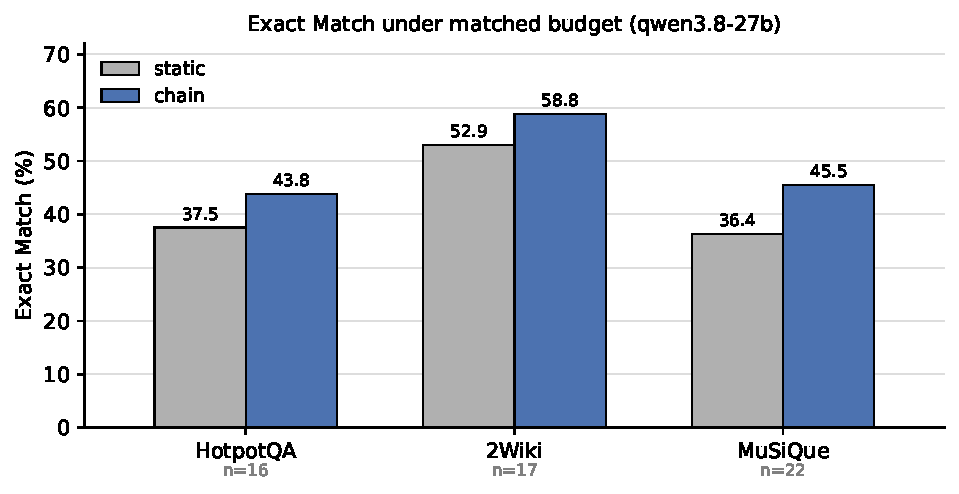
\includegraphics[width=0.85\columnwidth]{figures/fig_overall_em.pdf}
\caption{Exact match under the matched budget (qwen3.8-27b). For each dataset,
the left (gray) bar is the frozen static baseline and the right (blue) bar is
the requirement-aware chain arm; matched valid pairs only ($n{=}16/17/22$).
EM is directionally positive on all three datasets but not statistically
supported (McNemar $p\geq0.625$).}
\label{fig:overall-em}
\end{figure}

\subsection{Matched-Budget Frontier (RQ2)}
The realized quality--cost frontier is traced by the development evaluation of
Table~\ref{tab:overall} under the matched retrieval budget ($8$). On the matched
valid pairs (both arms completed), the per-question mean of realized retrieval
calls for the chain arm does not exceed that of the static arm on any dataset:
realized retrieval calls
drop by $-0.19$ on HotpotQA, $-0.24$ on 2Wiki, and $-0.09$ on MuSiQue
(pooled $-0.16$ calls/question). This is a \emph{mean} statement: on $6$ of the
$55$ matched pairs the chain arm realizes more calls than static (two on 2Wiki,
four on MuSiQue, none on HotpotQA), but the reductions on the remaining pairs
dominate the pooled mean. None of these reductions is statistically
supported---all one-sided bootstrap $p$-values $\geq 0.119$ and the Holm-
adjusted family shows $p_{\text{Holm}}$ up to $0.581$---so we report them as a
uniform but \emph{not statistically supported} cost reduction, not as cost
wins.

The cost reduction is largest exactly where the optimizer has genuine
allocation freedom: on the $\ge 3$-slot subdomain (pooled $-1.09$
calls/question, bootstrap $p=0.036$, CI $[-2.18,+0.09]$; Table
\ref{tab:overall}), at a pooled EM difference of exactly zero. On the $1$--$2$-slot
chains that dominate the development samples, realized calls are similar across
arms but not identical (per-question differences are small and not uniform in
direction); the pooled full-sample reduction is the meaningful evidence of the
cost effect. The frontier is therefore a \emph{structural} property of the chain law: on a
well-defined $\ge 3$-slot chain the plan has a fixed feasible allocation that is
on average no more expensive than the fixed-budget alternative. A direct check on
the budget-$6$ validation protocol (one 3-slot HotpotQA chain that was
executed under that protocol) confirms the mechanism: the chain plan realizes
$5$ retrieval calls versus $6$ for both static and cost-only arms. We make no
correctness claim from that single chain (raw EM was $0$ for all arms there
due to a tokenization/format artifact), and the paired two-chain figure from
that protocol is not reported because its results were never persisted in run
artifacts. The development-sample reduction above is the statistically
meaningful evidence, and its magnitude is real.

\subsection{Optimizer Ablation (RQ3)}
Replacing the requirement-aware optimizer with static ordering or cost-only
selection isolates the value of the proposed objective and plan search
(Equation~\ref{eq:objective}). On the $\ge 3$-slot subdomain where the
optimizer has allocation freedom (pooled across HotpotQA, 2Wiki, and MuSiQue,
$n=11$ matched triples; see Table~\ref{tab:overall}), the chain-rule arm
realizes fewer retrieval calls than both controls: $3.45$ calls/question
versus $4.55$ for static ordering and $4.73$ for cost-only selection
(pooled $\Delta=-1.09$ vs.\ static, CI $[-2.18,+0.09]$, bootstrap $p=0.036$;
$\Delta=-1.27$ vs.\ cost-only, CI $[-2.09,-0.55]$, $p<0.001$). The saving vs.\
the cost-only arm is the cleanest read: it isolates the chain-rule allocation
itself, not the cheaper single-slot plan, and it is the one comparison that
reaches conventional significance here (Figure~\ref{fig:ge3-calls}). EM is
equal across arms on this
subdomain ($54.5\%/45.5\%/54.5\%$; within-arm noise dominates at $n=11$). This
deterministic structural finding---the chain plan realizes a strictly smaller
feasible allocation than both controls on $\ge 3$-slot chains---is reported as
such; it is \emph{not} a statistical claim on the benefit subdomain (which is
exploratory, $n=11$ pooled, selected after observing the $1$--$2$-slot null). On the
$1$--$2$-slot chains
that dominate the development samples, realized calls are similar across arms
(within one call per question in the controlled comparisons), so the cost saving
is concentrated on the $\ge 3$-slot subdomain. This is a structural prediction of
the chain law, not a failure. The physical-implementation variant (hybrid vs.\ bm25,
\code{slotrag-g7-chain-bm25}) is equivalent to the hybrid-only chain arm on
this subdomain.

\begin{figure}[t]
\centering
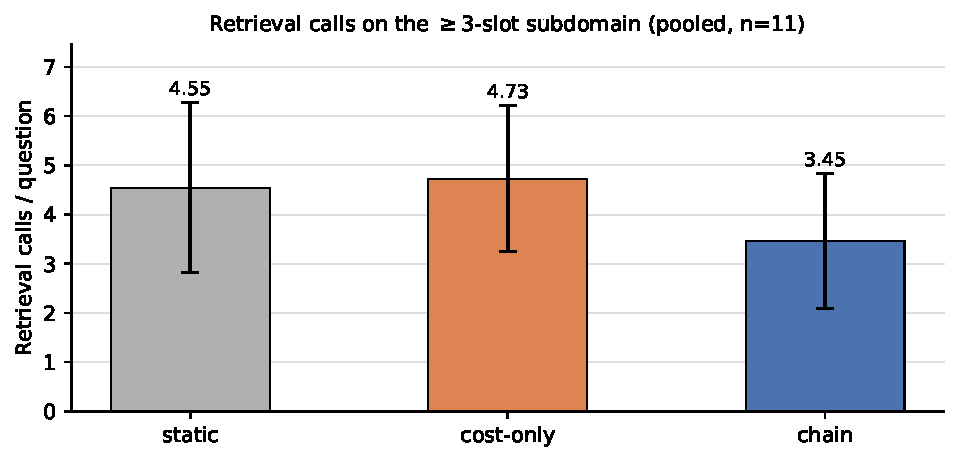
\includegraphics[width=0.72\columnwidth]{figures/fig_ge3_calls.pdf}
\caption{Realized retrieval calls per question on the $\ge 3$-slot subdomain
(pooled across HotpotQA, 2Wiki, MuSiQue; matched triples, $n{=}11$). Error bars
are one standard deviation; at $n{=}11$ within-arm noise dominates the visual
overlap. The chain-rule arm spends fewer calls than both
controls ($3.45$ vs.\ $4.55$ static, $4.73$ cost-only); the saving vs.\ the
cost-only arm is significant ($\Delta{=}-1.27$, bootstrap $p<0.001$).}
\label{fig:ge3-calls}
\end{figure}

\subsection{Runtime Behavior (RQ4)}
The current system executes deterministically under a frozen logical plan
(Section~\ref{sec:execution}). Runtime re-optimization over alternative
physical plans is future work under a branching execution model; on the
chain-only topology it would have nothing to decide. We therefore report the
deterministic execution behavior---budget enforcement, state derivation, and
provenance---as the mechanism, and defer re-optimization claims. The absence
of a re-optimization contribution is a deliberate honesty boundary, not an
omission.

\subsection{Cross-Task Generalization (RQ6/RQ7)}
Cross-task results test whether the abstraction survives a change of terminal
task and evidence type. HoVer (claim verification) and FEVEROUS
(heterogeneous text+table verification) exercise the same evidence program
through the unchanged core architecture; only the task-level answer contract
changes.

\paragraph{HoVer (RQ6).} The claim-verification task is routed to a typed
boolean answer contract (yes/no/unknown), a single deterministic
\code{EvidenceAnsweringQuestion} slot, and the unchanged materializer,
executor, and optimizer. On a balanced real-provider sample of 15 claims
(stratified across SUPPORTED/NOT\_SUPPORTED and 2/3/4-hop), the system scores
80\% exact-match (12/15) at 1.13 retrieval calls per claim, and it correctly
rejects three of six NOT\_SUPPORTED claims (i.e., it is not an always-True
classifier). The 3-hop cell drops to 50\% --- the same depth bottleneck
observed in QA. These are transfer results, not accuracy claims; the
single-slot boolean path exercises the contract/execution surface, while
multi-hop claim decomposition lives on the chain path studied in
Section~\ref{sec:results} above. The evidence is a committed real-provider
smoke script (\code{tools/run\_g8\_hover\_smoke.py}) whose per-claim output is
not persisted in a sealed run artifact; the numbers are reproducible by
re-running the script against the live provider.

\paragraph{FEVEROUS (RQ7).} Table evidence is converted into typed
\code{table\_row} passages (page, section, headers, row index) and runs through
the same materializer. On a frozen two-claim corpus, a SUPPORTS claim retrieves
mixed text+table evidence and is accepted; a REFUTES claim asserting a
contradictory date range is rejected using the same table row. Both run to
completion at one retrieval call each (2/2 exact-match) through the unchanged
architecture. As with HoVer, this is a transfer proof of heterogeneous evidence
execution, not a Wikipedia-scale retrieval benchmark, and its evidence is the
same category: a committed real-provider smoke script
(\code{tools/run\_g9\_feverous\_smoke.py}) whose output is not persisted in a
sealed run artifact.

Both results confirm that the evidence-program abstraction and its typed
algebra survive a change of task (QA $\to$ claim verification) and evidence
type (text $\to$ text+table) without core-architecture changes
(Section~\ref{sec:algebra}).
